\documentclass[11pt,article,oneside]{memoir}
\usepackage{org-preamble-xelatex}
\input{vc}


\usepackage{graphicx}
% We will generate all images so they have a width \maxwidth. This means
% that they will get their normal width if they fit onto the page, but
% are scaled down if they would overflow the margins.
\makeatletter
\def\maxwidth{\ifdim\Gin@nat@width>\linewidth\linewidth
\else\Gin@nat@width\fi}
\makeatother
\let\Oldincludegraphics\includegraphics
\renewcommand{\includegraphics}[1]{\Oldincludegraphics[width=\maxwidth]{#1}}

\title{\bigskip \bigskip Introduction}
 
\author{\bigskip\Large }

\begin{document}  

\setsansfont[Mapping=tex-text, BoldFont={* Bold SemiCondensed}, ItalicFont={* Semibold SemiCondensed Italic}]{Myriad Pro}
\setmonofont[Mapping=tex-text,Scale=MatchLowercase]{Consolas}
\setromanfont[Mapping=tex-text,Numbers=OldStyle]{Minion Pro}


\setkeys{Gin}{width=1\textwidth}  
\setromanfont[Mapping=tex-text,Numbers=OldStyle]{Minion Pro} 
\setsansfont[Mapping=tex-text]{Minion Pro} 
\setmonofont[Mapping=tex-text,Scale=0.8]{Consolas}
\chapterstyle{article-4} 
\pagestyle{kjh}

\published{Draft only. Please do not cite without permission.}

\maketitle


\begin{quote}
``The pioneer spirit is still vigorous within this nation. Science
offers a largely unexplored hinterland for the pioneer who has the tools
for his task. The rewards of such exploration both for the Nation and
the individual are great. Scientific progress is one essential key to
our security as a nation, to our better health, to more jobs, to a
higher standard of living, and to our cultural progress.''

--- Vannevar Bush, \emph{Science: The Endless Frontier} (1945)\footnote{Vannevar
  Bush, \emph{Science: The Endless Frontier} (Washington, D.C.: U.S.
  Government Printing Office, 1945), vi.}
\end{quote}

\begin{quote}
``Palo Alto is half bedroom suburb, half futuristic 1970s science
fiction movies. . . . The big thing about Palo Alto is that, as a city,
it designs tons of incredibly powerful and scarry shit inside its
science parks, which are EVERYWHERE.''

--- Douglas Coupland, \emph{Microserfs} (1995)
\end{quote}

\begin{quote}
``The underlying principle of conservation has been described as the
application of common sense to common problems for the common good. If
the description is correct, then conservation is the great fundamental
basis for national efficiency. In this stage of the world's history to
be fearless, to be just, and to be efficient are the three great
requirements of national life. National efficiency is the result of
natural resources well handled, of freedom of opportunity for every man,
and of the inherent capacity, trained ability, knowledge and will,
collectively and individually to use that opportunity.''

Theodore Roosevelt (1909)
\end{quote}

Paulina Borsook could no longer recognize her home city of San
Francisco. Surveying the ``Internetting of San Francisco'' in 1999, she
bemoaned the growth of condos, the increasingly poor parking, the fading
kindness she often experienced among strangers on the street, and the
endless grind of work. To her great concern, San Francisco was ceding
its ``unique history and sensibility'' to ``twerps with `tude,
characterized by''speed, libertarian ethos, {[}and the{]} irritating
hipster pose" of ``22-year-old Barbie-bunny marketing girls who don't
realize the Web is not the Internet, and guys who have come to San
Francisco because the dot-com version of Dutch tulip-mania offers better
odds of instant wealth than making partner at Merrill Lynch.''\footnote{Paulina
  Borsook, ``How the Internet ruined San Francisco,'' \emph{Salon},
  October 28, 1999, http://www.salon.com/1999/10/28/internet\_2/.}

Borsook reacted as many in the San Francisco Bay Area had to the
profound urban changes that the information sector had introduced. No
area of the Bay was more affected by high technology than the Santa
Clara Valley, what would become known as Silicon Valley in the 1970s.

At the close of World War II, Vannevar Bush, director of the Office of
Scientific Research and Development, issued a report to the president
titled \emph{Science: The Endless Frontier} urging continued federal
investment in scientific research to promote economic development and
national defense. Government officials heeded Bush's urgings and during
the Great Boom between 1940 and 1975 Western North America would be
profoundly influenced by the United States' interests in scientific and
military research. The twentieth-century American West, according to
Kevin Fernlund, ``bristled with airfields, army bases, naval yards,
marine camps, missile fields, nuclear test sites, proving grounds,
bombing ranges, weapons plants, military reservations, training schools,
toxic waste dumps, strategic mines, transportation routes, lines of
communication, laboratories, command centers, and arsenals.''\footnote{Kevin
  J. Fernlund, ed., \emph{The Cold War American West, 1945-1989}
  (Albuquerque: University of New Mexico Press, 1998), 1.} In addition,
the new economy of digital technology and electronics research and
development would influence urban change in the West's metropolitan
areas.

When the popular culture and technology pundits think of computers
today, the focus is often on San Francisco Bay Area innovators and
Seattle Microsoft billionaires. But the story of the silicon frontier
encompasses a much bigger pool of innovation and investment, namely from
government and university funding of early computing and computational
research. Federal funding awarded to western universities, where much of
the Cold War science innovation would take place, meant significant
changes to the military-metropolitan-technological matrix resulting in
expanding populations and increasing funding and reputations of western
research universities. Investment into digital computing and electronics
research allowed western universities to establish themselves while also
contributing to the cementing of the academic-military-industrial
complex in the region.

The militarization of science would have far reaching consequences for
the American West. Historians Richard White, Gerald Nash, Richard
Etulain, Carl Abbott, and others have noted the importance of defense
spending and computers in the American West, but no western historians
have contributed to a sustained examination of what the electronics
infrastructure meant for the region. The aerospace and computer
industries found homes in the West. California had 24\% of the prime
military contracts in the country in 1959. In 1962, the Pacific Coast
had 46\% of all Defense Department contracts for research and
development. The interior states of the West also increased their ties
to the growing military-industrial complex, and these industries
attracted a better-educated workforce and urban populace: The service
economy required an educated workforce and the urban regions of the
West, both by attracting educated migrants and investing in educational
systems proved capable of providing it. Urban westerners were better
educated than Americans overall: almost 46\% of the adults in the
metropolitan regions of the West were high school graduates in 1950,
compared to 34.3\% in the rest of the nation. As the national average
rose over the next two decades the West maintained its 10\% edge. In
1960, Albuquerque, New Mexico, boasted more Ph.D.~degrees per capita
than any other American city.

\begin{center}\rule{3in}{0.4pt}\end{center}

The networks and digital technology that characterize much of our lives
today obscures the physicality of technology. Paul Edwards, a historian
of computers in the Cold War, notes that the ``process is not only
technical, but also commercial, social, and political. It opens the door
to integrated infrastructures of huge scale and scope.'' The virtual
environments are rooted in physical space, and these spaces depend on
technologies as varied as underground fiber optic cables, microwave
transistors, and suburban offices.

The story told here approaches the history of the Internet from a
different perspective. Histories of the Internet tend to emphasize the
pioneers and technologies that formed the basis of the network: Vint
Cerf, Bob Taylor, ARPANET, TCP/IP, and so on. The story I seek examines
the process surrounding the Internet from a different perspective.
Rather than viewed as a history of technology or an examination of the
social underpinnings that are embedded in the Internet's design, I look
at how those attracted to the technology industries in the American West
contributed to the process of suburbanization. The Internet and its
creators, in fact, take a back seat in the story. The arrival of
thousands of scientists, engineers, and graduate students to research
institutions who were working on electronics research and development
introduced wide-ranging changes in the urban, demographic, and political
make-up of these silicon cities.

Part of the story has been told by others. Margaret O'Mara and John
Findley have written the best accounts of Silicon Valley and its place
in urban processes. But their stories focus on the institutional and
cultural construction of Silicon Valley from the perspective of those
\emph{doing} the building. My story examines those affected \emph{by}
the building of Silicon Valley. City leaders, residents, laborers,
migrant workers, and others all experienced rapid urban change after
World War II and responded in various ways to these changes.

The story told here stands at the intersections of postindustrial
society, political mobilization of racial and middle-class
neighborhoods, and the spatial politics of suburbanization and economic
development in the Far West. The temporal and regional scope of this
project begins in World War II, in the midst of urban restructuring and
economic transformations, and follows the story through the Cold War in
Santa Clara County, California, and Salt Lake County, Utah. These two
places had become key leaders in electronics research and development,
so much so that they were chosen as sites for the original four nodes of
ARPANET.

Part of what made Utah and California key players in high technology was
their status as ``cities of knowledge'' that relied on major research
universities as engines of economic development. Major studies on the
transformations of research universities during the Cold War have tended
to view the changes from inside the university while embracing broader
scholarly debates about scientists and American politics in the Cold
War. Authors have reached differing conclusions, on the one hand
emphasizing how federal policies left university administrators little
room for maneuverability and choice in adopting sweeping changes, and on
the other that university administrators eagerly accepted new
opportunities and willingly reorganized their institutions.\footnote{University-centered
  studies include Rebecca Lowen's \emph{Creating the Cold War
  University: The Transformation of Stanford} (1997), Roger L. Geiger's
  \emph{Research and Relevant Knowledge: American Research Universities
  since World War II} (1993), and Stuart W. Leslie's \emph{The Cold War
  and American Science: The Military-Industrial Complex at MIT and
  Stanford} (1993). The rise of scientific professionalization and
  expertise is explored in Jessica Wang, \emph{American Science in an
  Age of Anxiety: Scientists, Anticommunism, and the Cold War} (1999),
  Daniel J. Kevles, \emph{The Physicists: The History of a Scientific
  Community in Modern America} (1995), and Brian Balogh, \emph{Chain
  Reaction: Expert Debate and Public Participation in American
  Commercial Nuclear Power, 1945-1975} (1991).} Margaret O'Mara's
comparative history examining the growth of ``knowledge suburbs'' in the
Cold War most clearly traces how the confluence of white collar workers,
scientists and engineers, and research universities led some cities to
pursue high technology as a mechanism for economic growth.

This study fills in important gaps about the history of Silicon Valley,
focusing on those affected \emph{by} the building rather than those
\emph{doing} the building.

It also builds upon important work about urban history and grassroots
politics.

Three themes connect the local communities under study to broader
national trends. First, emerging from World War II, California and Utah
typified metropolitan transformation in contrast to the declining
industrial economies in the Northeast and Midwest. Santa Clara County
and Salt Lake County came to dominate cultural and commercial influence
in the United States, becoming what Carl Abbott called the ``new centers
for American life.''\footnote{Abbott, ``The Metropolitan Region,''
  p.~90.} Second, the migration of new middle-class workers to the
burgeoning computer economy in the West led to clashes between existing
residents and newcomers. The migration of people to Silicon Valley and
Salt Lake City pushed long-time residents out of city centers and
suburbs and displaced traditional labor markets in agriculture, mining,
and meatpacking. Finally, the rise of the metropolitan West occurred
just as the New Deal Order experienced collapse and in its place
conservatism rose ascendant.

The story here is about grassroots politics in suburban development and
the interplay between local and national\ldots{}

These urban processes are backdropped by the Cold War defense
imperative.

\begin{figure}[htbp]
\centering
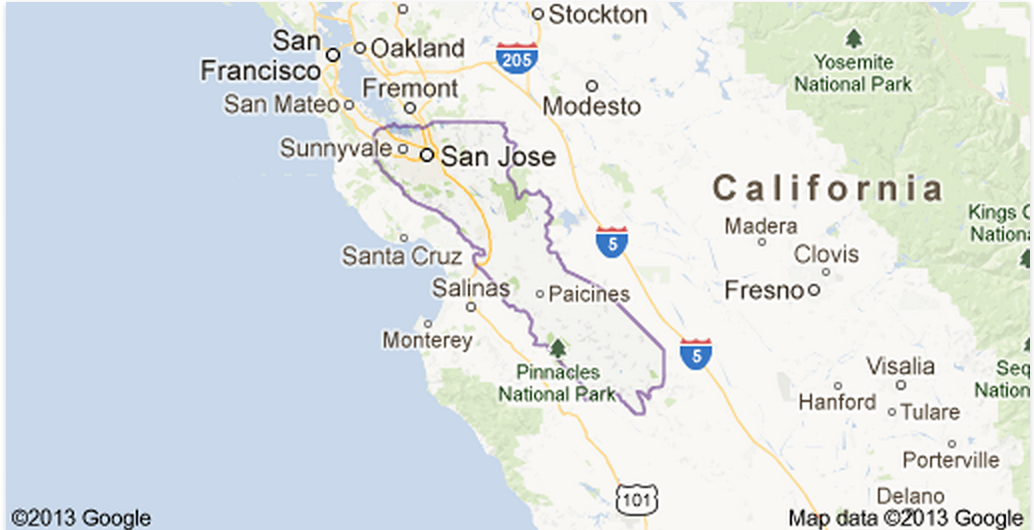
\includegraphics{/Users/jheppler/Projects/Dissertation/figures/sv.png}
\caption{Silicon Valley. The Santa Clara Valley lies between the Santa
Cruz Mountains on the west and the Diablo Range to the east, largely
encompassing the municipalities of San Jose, Mountain View, Sunnyvale,
Palo Alto, Menlo Park, and Redwood City. Between 1945 and 2000, San Jose
became the largest city in the Bay Area and ranked the near the top of
population growth in the nation.}
\end{figure}

Metropolitan growth, annexations, and and incorporations were so rapid
that Robert Self called the process a ``land rush.''\footnote{Self,
  \emph{American Babylon}, 120.}

The study approaches political history at the local level. City leaders,
activists, residents, and so on shaped the implementation and
interpretation of policies \ldots{}

The story also recounts a history of American politics in the
mid-twentieth century and the role of capitalism in shaping ideas. {[}As
Robbins notes, capitalism is more than economics but also reflects an
ideology and view about the world.{]} Several scholars have looked to
business and capitalism fueling a rise in conservatism, seeing Sunbelt
growth and defense-dependent economies becoming strongholds for
political conservatism.\footnote{Ann Markusen, et al., \emph{The Rise of
  the Gunbelt}; Bruce Schulman, \emph{From Cotton Belt to Sunbelt}; Lisa
  McGirr, \emph{Suburban Warriors}; Michelle Nickerson and Darren
  Dochuk, eds., \emph{Sunbelt Rising}; Bethany Moreton, \emph{To Serve
  God and Walmart}.} But the opposite holds true for the Valley. By the
1990s, Democrats saw the entrepreneurs of Silicon Valley as part of the
``New Democrats'' espoused by Bill Clinton, Al Gore, and others,
predicated on an orientation towards business, globalization, racial
diversity, cultural libertarianism, and meritocracy.\footnote{Sara
  Miles, \emph{How to Hack a Party Line: The Democrats and Silicon
  Valley} (University of California Press, 2002).} The language of
business, capital, labor, and markets became central to defining Silicon
Valley --- what historian Daniel Rodgers called a ``revival of market
ideology'' --- and maintained that capitalism would solve inequality and
poverty.\footnote{Daniel T. Rodgers, \emph{Age of Fracture} (Cambridge:
  Harvard University Press, 2011).}

Although the story told here is situated in a local environment dealing
with specific people reacting to local politics, the story of Santa
Clara County has broader implications for the history of postwar US
history. The process of suburbanization\ldots{}. Silicon Valley also
reflects a growing political reaction to capitalism\ldots{} The flow of
capital, labor, and knowledge into the Valley introduced profound
changes in the way people perceived space around them and related to one
another.

--

In examining the human and environmental costs of water, electronics,
outdoor recreation, urban development, and wilderness areas, this study
evaluates the costs of these programs. Although this study is tightly
focused on a specific region, it has greater bearing on understanding
the inherent tension between local and national politics. In the Santa
Clara Valley, the development of new landscapes, resulting from various
perceptions of the region as farmland, electronics manufacturer, urban
oasis, and tourist destination shaped the use of water in the valley.

Water and technology are icons in California. The battle over the Hetch
Hetchy reservoir and the growth of environmentalism calls to mind the
importance of water and its battles in the Far West, while the
electronics industry has located its origin myth in the former orchard
fields surrounding Stanford University. These two icons share the
California landscape in ways not yet examined by historians. Although
considered separate landscapes, they are entangled in ways not
previously understood. Water and the Santa Clara Valley share what
Richard White has called a hybrid landscape. Neither rural or urban,
hybrid landscapes are complex creations of natural and cultural systems
that shape a place.\footnote{Richard White, ``From Wilderness to Hybrid
  Landscapes: The Cultural Turn in Environmental History,'' \emph{The
  Historian} 66 (September 2004): 562-664.}

Water became a linchpin in contests over power conflicts: who controlled
water, who had access to water, how water should and could be used. The
valley's agricultural past required access to water to support orchard
fields. Later in the twentieth century, water became key to
semiconductor manufacturers, who used an ultra-purified water in the
process of manufacturing electronics components. Supporting urban growth
offered a third theme in contests over water, as the valley's population
exploded in the mid-twentieth century. And finally, residents new and
old made demands on water as recreation. Dam projects by the state of
California in and around the Santa Clara Valley became tied to
recreation and tourism while simultaneously supporting other water
projects for manufacturing and urban growth.

Efforts by federal regulators, city officials, business leaders, and
farmers all attempted to maximize their access to water. Beginning in
the 1930s, orchard fields in the Santa Clara Valley became national
producers of prunes, cherries, avocados, \{more\}. The growing
agribusiness presence in the Bay Area made demands on local water
resources and led federal officials and state political leaders to
pursue water and irrigation projects that would sustain farmlands. Yet
by the 1930s so much water was being pumped out of underground water
basins that Stanford geologists discovered that Santa Clara Valley had
sunk four feet in just twenty years.\footnote{``Data Show Sinking of Bay
  Area,'' \emph{Los Angeles Times} March 20, 1934, p.~1. The process of
  land sinking is known as subsidence and results from the weight of
  land compacting underground sand and gravel acquifers that have been
  drained. Subsidence would not end until 1969. By then, downtown San
  Jose had sunk ten feet and Alviso had sunk thirteen feet.} Concerns
over the Valley's access to water led to the development of the Central
Valley Project in the late 1930s.

South Bay Aqueduct and San Joaquin Valley Project, along with San
Francisco's Hetch Hetchy reservoir, supplied over half the water to the
Valley. The water projects were essential to support the growing
suburbs, high tech industries, and agriculture in the Valley.

The story here resituates how we understand Silicon Valley by placing
the environment at the core of the story. \{expand\}

\subsubsection{The Bay Area}

The San Francisco Bay Area is among the most highly populated places in
the United States. The area is physiographically situated between the
Santa Cruz mountains to the west and the Diablo Range to the east, a
tightly compact area spanning only \{MILES\} across and \{MILES\} long.
Hydrologically, the region is fed by several rivers and aquifers
dominated by the \{FACT\}.

\begin{figure}[htbp]
\centering
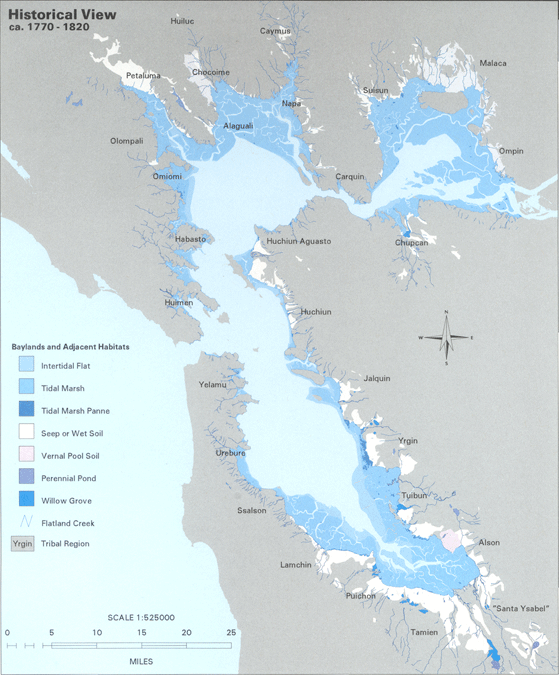
\includegraphics{/Users/jheppler/Projects/Dissertation/figures/hydrology.png}
\caption{Bay Area hydrology}
\end{figure}

The Internet maintains such a large scope in our lives today with its
near ubiquity in wireless networks and smart phones, but this obscures
the technology's physical foundation. As Paul Edwards notes, the
``process is not only technical, but also commercial, social, and
political. It opens the door to integrated infrastructures of huge scale
and scope.'' (Edwards, ``Y2K: Millennial Reflections on Computers as
Infrastructure,'' \emph{History and Technology} 15 (1998): 16). The
electronic spaces of the Internet are indeed virtual, but these virtual
environments are rooted in a physical world. These electronic spaces
depend on underground fiber optic tables, microwave transistors,
suburban offices where administrators monitor networks.

\subsubsection{The Landscape of Conflict}

Geographer John Wright argued that ``places are best seen as shifting
stages where the exercise of power and resistance to it vie for
dominance.''

--

The story I tell can be found in other works: Margaret O'Mara and John
Findley, for example. But their stories focus on the institutional and
cultural construction and meaning of Silicon Valley. The story I seek to
tell places these stories on the periphery, and instead I focus on a
micro view of urban change and interpersonal networks that formed in
response to these changes. City leaders, residents, laborers, migrant
workers, and others all experienced rapid urban change after World War
II and responded in various ways to these changes. In particular, my
work focuses on areas where the rise of the computer economy had the
greatest impact.

The computer economy, defined here, is broadly encompassing: the
university, research and development, scientific experimentation,
nuclear testing, space flight, aerospace, etc. all felt the influence of
computer technology.

These urban changes and new economies are backdropped by the Cold War.

--

Silicon Valley was an imagined community.

\begin{center}\rule{3in}{0.4pt}\end{center}

The story told here stands at the intersections of postindustrial
society, political mobilization of racial and middle-class
neighborhoods, and the spatial politics of suburbanization and economic
development in the Far West. The regional scope of this project begins
in World War II, in the midst of urban restructuring and economic
transformations, and follows the story through the Cold War in Santa
Clara County, California, and Salt Lake County, Utah.

Three themes connect the local communities under study to broader
national trends. Emerging from World War II, California and Utah
typified metropolitan transformation in contrast to the declining
industrial economies in the Northeast and Midwest. Simultaneously, the
migration of new middle-class workers to the burgeoning computer economy
in the West led to clashes between minority residents and newcomers. The
migration of people to Silicon Valley and Salt Lake City pushed
long-time residents out of city centers and suburbs. Finally, the rise
of the metropolitan West occurred just as the New Deal Order experienced
collapse and in its place conservatism rose ascendant.

The story here is about grassroots politics in suburban development and
the interplay between local and national in the emergence of the
center-right politics that has come to dominate American politics since
the 1960s. Most works on conservatism have examined the Southern
Strategy of Richard Nixon

Lotchin argues that leaders used federal resources to build urban
empires and military complexes, which increased the flow of federal
dollars into the state. O'Mara demonstrates how Stanford did this in SV.

--- A rural history of Silicon Valley? - Farmers, workers, and
metropolitan space in santa clara valley as a theme\ldots{}

\subsection{Postwar Western Demographics}

The mobilization of the country in World War II dramatically altered the
nation and people's daily lives. Following a decade of economic
depression, people migrated to metropolitan areas to take new wartime
industries. The American West especially felt the impact of this
demographic shift, leading Carl Abbott to remark that launched ``the
entire West into the half-century of head-long urbanization.''\footnote{Abbott,
  \emph{Metropolitan Frontier}, p.~4.} Six of the largest western
metropolitan areas in 1940 grew by 380\% over the course of fifty years,
compared to just 64\% for the six largest in the East.\footnote{Abbott,
  \emph{Metropolitan Frontier}, p.~xiii.} Just as populations were
migrating to metropolitan centers, the number of people living inside
city boundaries was declining. The attraction of suburban life

\begin{enumerate}[(1)]
\setcounter{enumi}{146}
\item
  ``massive military expenditures have spurred a major spatial shift in
  manufacturing production to the so-called defense perimeter. In this
  manner, the federal government, by means of its military budget and
  locational preferences, has promoted uneven regional development.''
\item
  ``At the center of these processes of economic structuring and spatial
  shifts is the information sector, which includes both information
  technologies (the hardware part) and the use of advanced information
  systems (the software part). The spatial consequences of these
  information technologies and systems deserve more attention from
  historians than they have received. Introduction of these new
  technologies in the manufacturing and service sectors, for example,
  directly affects where businesses choose to locate -- since it reduces
  the need for spatial proximity.''
\item
  Sees Orange County as a leader in these processes -- economic
  restructuring, militarization of production, spatial transformation,
  information technologies and systems, internationalization of a
  regional economy. --- Olin article (above)
\end{enumerate}

Although there is a widening historiography on the influence of science,
military funding, and government presence on the twentieth century
American West, very little of this literature has addressed the
influence of computing and electronics research and entrepreneurship and
its role in shaping the New West. My project brings together literatures
in urban, technological, and institutional history in the West to
describe the goals and outcomes of urban policies and university
politics. Discussions of the causes behind the West's urban growth have
tended to examine political and social change in individual cities and
compare these developments to other examples of metropolitan
development. Issues of location, metropolitan size, age, history of
growth, economic environment, and location have been identified by
researchers as important to explaining differences and similarities
between western cities. Political change is a common framework in
assessing urban development. Roger Lotchin, John Mollenkopf, Carl
Abbott, and Peter Wiley and Robert Gottlieb have undertaken case studies
in studying individual industries and urban growth.\footnote{Roger
  Lotchin, ``The City and the Sword: San Francisco and the Rise of the
  Metropolian Military Complex, 1919-41,'' \emph{Journal of Americna
  History} 65 (March 1979): 996-1020; Lotchin, ``The Darwinian City: The
  Politics of Urbanization in San Francisco between the World Wars,''
  \emph{Pacific Historical Review} 48 (August 1979): 357-81; John
  Mollenkopf, \emph{Contested City}; Abbott, \emph{New Urban America};
  Wiley and Gottlieb, \emph{Empires in the Sun}.}

New work in urban history has explored how postwar suburbs were not
defined as unplanned suburbn sprawl but rather were planned communities.
Robert O. Self's American Babylon: Race and the Struggle for Postwar
Oakland (2003), Greg Hise's Magnetic Los Angeles: Planning the
Twentieth-Century Metropolis (1997), and Robert E. Lang's Edgeless
Cities: Exploring the Elusive Metropolis (2003).

Santa Clara County and Salt Lake County came to dominate cultural and
commercial influence in the United States, becoming what Carl Abbott
called the ``new centers for American life.''\footnote{Abbott, ``The
  Metropolitan Region,'' p.~90.}

At root, the project seeks to tell a story about the social, cultural,
and political changes that happened locally during the Cold War through
the lens of early historical developments in computing and federal
research and development.

Many works have outlined the mutual relationship between technology and
social institutions. Paul Edward's The Closed World: Computers and the
Politics of Discourse in Cold War America was the first to examine how
the military influenced computer design and how technical developments
influenced military institutions.\footnote{Gabrielle Hecht, \emph{The
  Radiance of France: Nuclear Power and National Identity After World
  War II} (1998), Donald MacKenzie \emph{Inventing Accuracy: A
  Historical Sociology of Nuclear Missile Guidance} (1990), and Ken
  Alder \emph{Engineering the Revolution: Arms and Enlightenment in
  France, 1763-1815} (1997) have also studied the relationship between
  new technology and social institutions.}

Major studies on the transformations of research universities during the
Cold War have tended to view the changes from inside the university
while embracing broader scholarly debates about scientists and American
politics in the Cold War. Authors have reached differing conclusions, on
the one hand emphasizing how federal policies left university
administrators little room for maneuverability and choice in adopting
sweeping changes, and on the other that university administrators
eagerly accepted new opportunities and willingly reorganized their
institutions. University-centered studies include Rebecca Lowen's
Creating the Cold War University: The Transformation of Stanford (1997),
Roger L. Geiger's Research and Relevant Knowledge: American Research
Universities since World War II (1993), and Stuart W. Leslie's The Cold
War and American Science: The Military-Industrial Complex at MIT and
Stanford (1993). The rise of scientific professionalization and
expertise is explored in Jessica Wang, American Science in an Age of
Anxiety: Scientists, Anticommunism, and the Cold War (1999), Daniel J.
Kevles, The Physicists: The History of a Scientific Community in Modern
America (1995), and Brian Balogh, Chain Reaction: Expert Debate and
Public Participation in American Commercial Nuclear Power, 1945-1975
(1991).

While the historiography on the relationship between universities and
the military is rich, less so are studies about what that relationship
meant for the metropolitan areas where such universities resided.
Margaret O'Mara's work \emph{Cities of Knowledge} is a recent example
examining how urban centers were shaped by, or served to shape,
universities and federal research and development dollars. My project
adopts O'Mara's ideas about cities of knowledge and applies them to
other institutions in California. How, for example, does private,
suburban Stanford compare to a public, suburban university of UCLA? How
do these other institutions, who do not become the next Silicon Valley,
seed high-tech reputations? How are these four universities chosen as
the original nodes of what would later develop into the Internet?

The spectrum of work on computer history tends to fall in one of two
camps: either on the technical side that nearly requires specialized
knowledge of computer science and engineering, or the popular
science/technology writing that treats the history as a progression of
inventions, biographies, and innovations. Books such as Katie Hafner and
Matthew Lyon's \emph{Where the Wizards Stay Up Late} chart the origins
of the Internet, but do not locate the story within a regional
context.\footnote{Historian Roy Rosenzweig provided an excellent early
  historiographical examination of the Internet in ``Wizards,
  Bureaucrats, Warriors, and Hackers: Writing the History of the
  Internet,'' \emph{American Historical Review} 103 (December 1998):
  1530-1552. Rosenzweig identified several patterns in the history of
  the Internet, noting that most studies fell within biographic,
  bureaucratic, social, and ideological frameworks. Rosenzweig concluded
  that new studies about the Internet needed to bridge biographical and
  institional histories and more fully contextualize social and cultural
  history. Recent works on the history of the Internet, including Johnny
  Ryan's \emph{History of the Internet and Digital Future} (New York:
  Reaktion Books, 2010), continues the trend of popular technology
  writing that focuses on ideas and biographies without much
  contextualization.} John Markoff's \emph{What the Dormouse Said} and
Fred Turner's \emph{From Counterculture to Cyberculture} do more to
locate the unique regional characteristics of the San Francisco Bay area
and the interplay of entrepreneurship and the counterculture in
envisioning the computer as a tool of liberation. What these studies
lack, however, is situating these histories into a broader Western
context that go beyond California history.

My study expands on the work of historians who have only begun to assess
the intermixing of universities, the military, and industry in the
American West after World War II and pushes the story beyond its popular
focus into bigger questions about the West's role in developing high
technology. The combination of entrepreneurial energy, government
investment, and university research led to explosive growth in the
information industry. The research, for government officials, was
literally life or death. Investment into high technology made national
security sense in the wake of the Soviet Union's acquisition of nuclear
weapons and launch of Sputnik. Keeping the technological edge over the
Soviets became a national security imperative. The American West served
this goal not only as a region for storing or testing nuclear weapons
and other defense-related material, but also served as a key region in
innovation and experimentation with digital computers--a story largely
unexplored by historians of the American West.

My study also contributes to the growing historiography on the domestic
Cold War and situates an everyday device----digital computers----as the
center of the story. The role of economic and political concerns to
national security strategy has generated wide analysis by political
scientists. My project also examines further the regional favoritism of
military spending identified by historians Bruce Schulman From Cotton
Belt to Sunbelt and Roger Lotchin's Fortress California.

\subsection{Organization}

The dissertation is organized chronologically and thematically. Each
chapter is roughly chronological to one another, but thematic in their
narrative to explore the various processes and contests at work in the
Valley. The themes are organized around irrigation, manufacturing,
tourism, and urban growth.

Chapter 1: The Western Water Landscape

Chapter 2: The Valley and the Future of the West

The dissertation is organized chronologically and thematically. Each
chapter is roughly chronological to one another, but thematic in their
narrative to explore the processes at work in the Santa Clara Valley.
The themes of the chapters are organized around biographies that
illustrate broader trends, as outlined below. I have identified enough
source material regarding these biographies to make such an approach
easily viable. The approach to using biographies is also unique, giving
various perspectives on the urban, political, and social changes
occurring in the Valley.

Instead of biographies framing entire chapters -- what if biographies
form interludes? e.g., the start of each part, perhaps, gets an
interlude about specific people and how they fit in with the larger
point of the chapters?

\textbf{Part 1: Visions}

Part One traces how different groups envisioned the future of the Santa
Clara Valley. Trade unionists, Latinos, African Americans, political
activists, suburbanites, and business leaders struggled to bring their
urban visions to life.

\textbf{Chapter 1: Staking the West's Future on Silicon Valley}

Influential leaders at Stanford University and Santa Clara Valley
business elites staked their future fortunes on Silicon Valley's
success. Surveying the declining Northeast and frustrated with the
West's status as a ``colony'' of the East, businesses in the Valley
sought ways to make a name for themselves. Frederick Terman, who served
as Stanford's Dean of Engineering and ostensible ``father of Silicon
Valley,'' experienced the electronics industry in the East during World
War II. Terman saw an opportunity for electronics research and
development that would bolster Stanford's reputation as a research
institution as well as open the American West to new economic
opportunities. Terman's plan for this process began in the
Stanford-owned lands near Palo Alto, but businesses specializing in
electronics quickly spread up and down the Bay. Chapter one sets the
stage, using Terman's biography as a lens to explore government,
university, and business interest in electronics research and
development. The Bay staked its future and opportunities on electronics
production.

\textbf{Chapter 2: Business in the Bay}

Chapter two narrates the story beyond Terman's ideas for Silicon Valley,
and discusses the role businesses played in shaping the political,
social, and economic structure of the Santa Clara Valley. The seedbed
for business growth was set in place by Terman, and businesses began
migrating to the Bay in large numbers. The Cold War industrial boom,
regional business entrepreneurs, and migrants attracted to the new high
technology industries changed the political and social face of the
Valley's municipalities. Chapter two uses Robert Noyce's biography to
explore the fortunes and tribulations of a single company--Noyce
Semiconductor--and the desires, opportunities, and conflicts embedded in
the company's establishment. The chapter will speak broadly as well
about the spread of businesses up and down the Bay who took advantage of
the offers made by Stanford and Bay Area municipalities seeking to
attract high technology to them.

\textbf{Part 2: Change}

Part two looks beyond the early stages of Silicon Valley to examine how
policies supported and created by planners, developers, university
administrators clashed with African Americans and Latinos in the Bay
Area who developed a different vision for the Valley. Ideas about
progress and opportunity were embedded in these clashing views.

\textbf{Chapter 3: ``Carved from a Forest of Fruit Trees'': Labor and
the Ideal of Progress in Santa Clara Valley\footnote{T. H. Bowden
  reported in his survey of San Jose that ``the city might literally be
  said to have been carved from a forest of fruit trees, as most of the
  residential sections were orchards prior to being subdivided and many
  of the original trees still ornament the gardens of the invading
  residences.'' Bowden, \emph{Report of a Survey in San Jose},
  California, 2.}}

Joe Ruscigno, a lifetime farmer and resident of the Valley, had taken up
a new occupation in 1952. ``Guess I've pulled out 150 acres of trees
since the first of the year,'' he told the \emph{San Francisco
Chronicle} as he sat atop his bulldozer next to a pile of uprooted fruit
trees. Ruscigno lamented the destroyed trees, but ``what can you do? . .
. The subdivisions were coming in all around us and when they made me a
good offer I sold out.''\footnote{``Santa Clara County --- Scene of the
  Big Boom,'' \emph{San Francisco Chronicle}, May 11, 1952.} The
Valley's suburbanization led to similar experiences as those by
Ruscigno.

The chapter will use Ruscigno's biography to explain broader changes
occurring throughout the Valley in the mid-1960s. As farms gave way to
suburbanization, so did livelihoods and labor change for migrant
workers, farm owners, electrical engineers, and scientists.

\{idea\} {[}Visualize the shrinking of the farms?\ldots{}{]}

\textbf{Chapter 4: Citizens in Action}

\textbf{Chapter 5: Seizing the Postwar Barrio}

In 1971, José Vasquez filed a lawsuit against the San Jose school
district on the grounds that his son, and other Chicano children,
discriminated against. ``We were the first people here,'' he argued.
``Someone else owned the land we worked; when the railroads came, we
didn't benefit. We never have. Then Silicon Valley came, and we never
shared in the prosperity. Why? Our kids are coming out of school and
they can't read; they can't get a job in Silicon Valley, and the schools
don't give a damn.'' Vasquez linked education and opportunity to Silicon
Valley.

Part 3: Attempts to manipulate the new urban West to their advantage.


\end{document}
